\chapter{Graphics}

The \jr\ provides three separate graphics engines, providing programs with a choice in how they display information to the user. Those different engines do share certain features, however, and this chapter will cover the common elements. The three graphics engines are bitmaps, tile maps, and sprites. What is common between all these elements is how they determine what colors to display and how to determine, when two or more objects are in the same place, which object is displayed.

\begin{itemize}
    \item Bitmaps are simple raster images. They are the size of the screen ($320 \times 200$ or $320 \times 240$) and cannot be moved. The TinyVicky chip used by the \jr\ allows for two separate bitmaps to be displayed at the same time.

    \item Tile maps are images made up of tiles. The tiles come in a tile set, which is a raster image like a bitmap but provides 256 tiles. The tile map itself creates its image by indicating which tile is displayed at every position in the tile map. This mapping can be changed on the fly, allowing tile maps to be altered, and tile maps can also be scrolled horizontally and vertically to a limited degree. This allows for possibility for smooth scrolling of a tile map scene. TinyVicky allows for three separate tile maps to be displayed simultaneously.

    \item Sprites are small, square graphics elements that may be moved to any position on the screen. Sprites are typically used to represent game characters or very mobile UI elements. TinyVicky sprites may be 8, 16, 24, or 32 pixels on a side. There may be as many as 64 sprites active on the screen at once (without using special techniques).
\end{itemize}

\section{Graphics Colors}

The graphics modes use a color lookup system similar to text mode to determine colors. The pixel data for a tile, bitmap, or sprite is composed of bytes, where each byte specifies the color of that pixel. The byte serves as an index into a color lookup table where the red, green, and blue components of the desired color are stored (see figure:~\ref{fig:bitmap_colors}). As with text, the color components are bytes and specify an intensity from 0 (none of that primary color) to 255 (as much of that primary color as possible). Also, as with text, there is a fourth byte that is reserved for future use, meaning that each color takes up four bytes in the CLUT. In short, the byte order of a graphics CLUT entry is exactly the same as for a text CLUT.

\begin{figure}[h]
    \begin{center}
        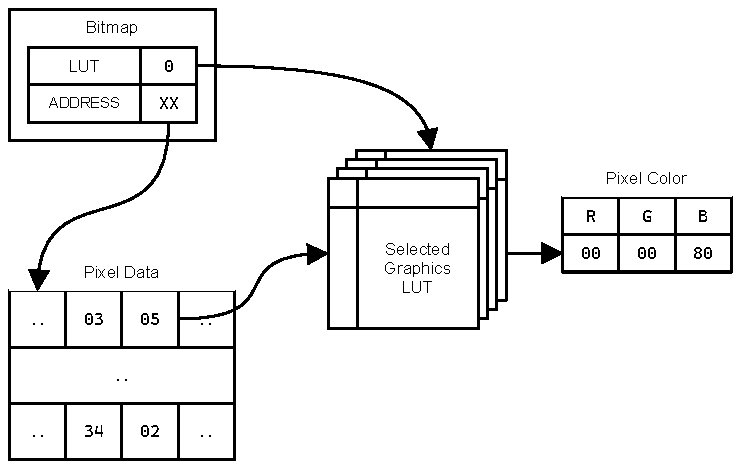
\includegraphics{images/bitmaps.pdf}
    \end{center}
    \caption{Bitmap Data to Pixels}
    \label{fig:bitmap_colors}
\end{figure}

However, there is a key difference from text mode. In text mode, there are two colors (foreground and background), and each color is one out of sixteen possibilities. With graphics modes, there are 256 possibilities. So a CLUT with only 16 entries will not work. There are therefore separate CLUTs for graphics. TinyVicky provides for four separate graphics CLUTs with 256 entries. Each graphic object on the screen specifies which graphics CLUT it will use for its colors. These CLUTs may be found in I/O page 0 (see table:~\ref{tab:graph_cluts}).

\begin{table}[h]
    \begin{center}
        \begin{tabular}{|c|l|} \hline
            Address & Purpose \\\hline\hline
            \verb+0xD000+ & Graphics CLUT 0 \\ \hline
            \verb+0xD400+ & Graphics CLUT 1 \\ \hline
            \verb+0xD800+ & Graphics CLUT 2 \\ \hline
            \verb+0xDC00+ & Graphics CLUT 3 \\ \hline
        \end{tabular}
    \end{center}
    \caption{Graphics Color Lookup Tables}
    \label{tab:graph_cluts}
\end{table}

\example{A Simple Gradient}

Let's set up a CLUT so that we have the colors for a gradient fill between red and blue. In this example, \verb+pointer+ is a two byte variable down in zero page, which will be used to point to the first byte of the CLUT entry the code is updating. The \verb+Y+ register is being used to point to the individual components of the entry.

\begin{verbatim}
MMU_IO_CTRL = $0001             ; MMU I/O Control Register
VKY_GR_CLUT_0 = $D000           ; Graphics LUT #0

;
; Initialize the LUT to greyscale from (255, 0, 0) to (0, 0, 255)
;

            lda #$01            ; Set the I/O page to #1
            sta MMU_IO_CTRL

            lda #<VKY_GR_CLUT_0 ; pointer will be used to point to a particular LUT entry
            sta pointer
            lda #>VKY_GR_CLUT_0
            sta pointer+1

            ldx #0              ; Start with blue = 0

lut_loop:   ldy #0              ; And start at the offset for blue
            txa                 ; Take the current blue color level
            sta (pointer),y     ; Set the blue component
            iny

            lda #0
            sta (pointer),y     ; Set the green component to 0
            iny

            txa                 ; Get the blue component again
            eor #$ff            ; And compute the 2's complement of it
            inc a
            sta (pointer),y     ; Set the red component
            iny

            inx                 ; Go to the next color
            beq lut_done        ; If we are back to black, we're done with the LUT

            clc                 ; Move pointer to the next LUT entry (+ 4)
            lda pointer
            adc #4
            sta pointer
            lda pointer+1
            adc #0
            sta pointer+1

            bra lut_loop

lut_done:
\end{verbatim}

\section{Pixel Data}

All three graphics engines arrange their pixel data in the same manner. They all use rectangular raster images as a base, although the width and height of the rectangle can vary. The pixels are placed in memory in sequential order in left-to-rigth and top-to-bottom order. That is, the first pixel in the sequence is the upper-left pixel in the image. The next pixel is the pixel to the immediate right and so on. If the image is $w \times h$, the position of a pixel at $(x, y)$ in the list is $y \times w + x$.

\section{Graphics Layers}

Now, what happens if two sprites take up the same position or if a program displays a tile map and a bitmap together? How does TinyVicky determine what color to display at a given position? TinyVicky provides a flexible layering system with several layers. Elements in ``near'' layers (lower numbers) get displayed on top of elements in ``far'' layers (higher numbers). If a sprite in layer 0 says a pixel should be blue while a tile in layer 1 says it should be red, the pixel will be blue. Color 0, however, is special. It is always the transparent ``color''. A pixel that is 0 in an element will be the color of whatever is behind it (or the global background color, if there is nothing behind it).

TinyVicky provides for seven layers, but they are split up a bit. Three of the layers are for bitmaps and tile maps. Only one bitmap or tile map can be placed in any of those three layers. The other four layers are for sprites only. Any sprite can be assigned to any of the sprite layers, and there can be multiple sprites in a layer. The sprite layers are interleaved with the bitmap and tile map layers (see figure:~\ref{fig:layers}).

\begin{figure}[h]
    \begin{center}
        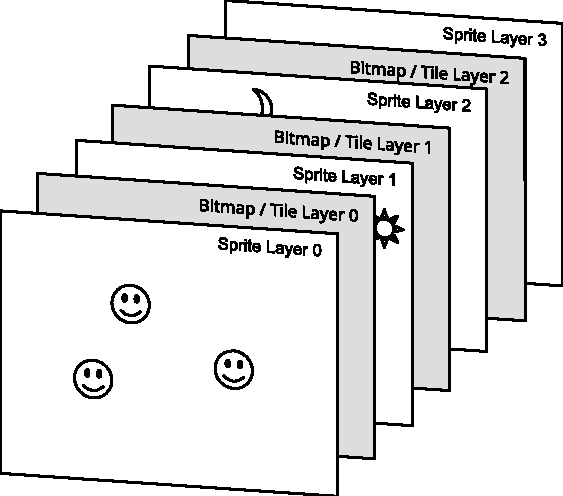
\includegraphics{images/Layers.pdf}
    \end{center}
    \caption{TinyVicky Graphic Layers}
    \label{fig:layers}
\end{figure}

Bitmaps and tile maps are assigned to their layers using the layer control registers (see table:~\ref{tab:bm_tm_layers}). The three fields LAYER0, LAYER1, and LAYER2 in the layer registers are three bit values, which indicate which graphical element to assign to that layer: 0--Bitmap 0, 1--Bitmap 1, 2--Tile map 0, 3--Tile map 1, 4--Tile map 2.

\begin{table}[h]
    \begin{center}
        \begin{tabular}{|c|c|c|c|c|c|c|c|c|} \hline
            Address & 7 & 6 & 5 & 4 & 3 & 2 & 1 & 0 \\ \hline\hline
            \verb+0xD002+ & --- & \multicolumn{3}{|c|}{LAYER1} & --- & \multicolumn{3}{|c|}{LAYER0} \\\hline
            \verb+0xD003+ & \multicolumn{5}{|c|}{---} & \multicolumn{3}{|c|}{LAYER2} \\\hline
        \end{tabular}
    \end{center}
    \caption{Bitmap and Tile Map Layer Registers}
    \label{tab:bm_tm_layers}
\end{table}

\example{Put Bitmap 0 on Layer 0}

As an example of how to use layers, we can set things up for future examples by putting bitmap 0 in the front layer (0), tile map 0 in the next layer (1), and bitmap 1 in the back layer (2).

\begin{verbatim}
    lda #$20            ; Layer 0 = BM 0, Layer 1 = TM 0
    sta VKY_LAYER_CTRL_0
    lda #$01            ; Layer 2 = BM 1
    sta VKY_LAYER_CTRL_1
\end{verbatim}
